\chapter{Background}

%============================= INTRODUCTION =================================
\section{Introduction}\label{sec:MLintro}
Artificial intelligence (AI) is a broad field that aims to develop intelligent
software that can e.g., acquire knowledge from its interaction with the world,
find optimized strategies for problem solving, automate tasks, detect patterns
in audio, video and textual data, play games, drive cars and much more.

Machine learning is a complex subfield of AI that witnessed a very quick
expansion in the recent years. It aims to enable computers to \emph{learn} how
to tackle problems by detecting patterns and regularities in the training data
and trying to generalize this extracted knowledge to new, unseen data.

Among its many powerful tools, artificial neural networks are models that take
inspiration from what we know about the human brain, by mimicking its
connectivity patterns, learning rules and signals propagation, under the
constraints imposed by out limited knowledge of the brain and a less powerful
hardware.

While it is beyond the scope of this document to give a formal and in-depth
introduction to every concept needed to fully comprehend Machine Learning,
the following sections will introduce Artificial neural networks, with a
specific focus on two of the most used kinds of neural networks. For a detailed
overview of Machine Learning, we suggest the interested reader to refer
to~\cite{bishop-book2006,Goodfellow-et-al-2016-Book}

%================================== SECTION ==================================
\section{Artificial neural networks}\label{sec:NN}
Brains are composed by a large amount of simple elements, called neurons,
that are highly interconnected. The number of neurons in the human brain is
estimated to be around $10^{11}$, each one connected to a little less than
$10^{4}$ other neurons, for a total between $10^{14}$ and $10^{15}$
synapses~\cite{drachman2005we}. The activity of each of these either excites or
inhibits the surrounding neurons it is connected to, generating a complex
network of interactions.

Artificial Neural Networks (ANNs) take inspiration from this understanding of
the human brain, building networks composed of many artificial neurons, small
elements that perform very simple operations on their inputs.

\subsection{Brief history of neural networks}
In 1943 McCulloch and Pitts defined a mathematical model of how a biological
neuron works~\citep{McCulloch43}. The artificial neuron they proposed was
able to solve simple binary problems, but did not learn. In 1949~\cite{Hebb49}
suggested that human learn by enhancing the neural pathways between neurons
that collaborate, and weakening the others. Only decades later this learning
rule inspired the Perceptron~(see~\autoref{fig:perceptron}), the first ANN that
was able to vary its own weights, i.e. to find the setting that allowed it to
exhibit the desired behavior~\citep{Rosenblatt57}.

% PERCEPTRON
\begin{figure}[h]
    \centering
    \begin{neuralnetwork} [nodespacing=6mm, layerspacing=23mm,
            maintitleheight=2.5em, layertitleheight=5em,
            height=3, toprow=true, nodesize=17pt,
            style={}, title={}, titlestyle={}]

        %%%%% Layers
        \inputlayer[count=5, bias=true, title=Input\\layer, text=\nodetextxi]
        \outputlayer[count=1, text=\nodetextsigma]
        {\setdefaultlinklabel{\wilink}\linklayers}
        \redefinelayerspacing{18mm}
        \outputlayer[count=1, text=\nodetextstep]
        \linklayers
        \redefinelayerspacing{16mm}
        \outputlayer[count=1, text=\nodetexty]
        \linklayers
    \end{neuralnetwork}
    \centering
    \caption{\label{fig:perceptron}A representation of the Perceptron.}
\end{figure}

The activation rule of the perceptron is very simple and is at the base of
many modern neural networks. Given an $n$-dimensional input $x$, the weighted
sum of each dimension of the input $x_i$ and its corresponding weight $w_i$ is
computed as

\begin{equation*}
    s = \sum_{i=0}^{n}(w_i \cdot x_i)
\end{equation*}

\noindent where to simplify the notation the bias term $b$ has been replaced
by an equivalent input term $x_0=b$. Note that this is simply the dot
product of the weight matrix $W$, frequently referred to as \emph{kernel}, and
the input vector $x$. The result of this first affine transformation is then
passed through a step function of form

\begin{equation*}
    y =
        \begin{cases}
            1,          & \text{if } s \geq 0 \\
            0,         & \text{otherwise}
        \end{cases}
\end{equation*}

% Although most modern ANNs apply a different nonlinear function
% (see~\autoref{sec:activation_fn}),
that determines the binary output of the Perceptron.

This is interesting because it can be used, e.g., to classify whether the input
belongs to a specific class or not, but the biggest innovation
of~\cite{Rosenblatt57} is most probably the update algorithm that allowed to
modify the weights of the model in a Hebbian rule fashion. The weights and the
bias -- also called the \emph{parameters} of the network -- are \emph{learned}
according to the following rule:

\begin{equation}\label{eq:perceptron_lr}
    w_i^{new} = w_i^{old} + \eta \cdot (\hat y - y) \cdot x_i
\end{equation}

\noindent where $\hat y$ is the target (i.e. desired) value, $y$ is the output
of the Perceptron, $x_i^t$ and $w_i^t$ are respectively the $i$-th input and
weight at time $t$ and $\eta$ is a scaling factor that allows to
adjust the magnitude by which the weights are modified.

The introduction of a model that could learn from the data
%This discovery
was welcomed with excitement as the beginning of a new era and
research in ANNs became very active for approximately a decade, until in
1969 Minsky and Papert published a detailed mathematical analysis of the
Perceptron, demonstrating that a single layered Perceptron could not model
basic operations like the XOR logic operation~\citep{Minsky69}. The limit of
Perceptrons is that they can only solve linearly separable problems, and fail
at tackling nonlinearly separable problems like the
XOR~(see~\autoref{fig:XOR}). This is not the case for MultiLayer
Perceptrons~(MLP, depicted in~\autoref{fig:MLP}), an evolution of Perceptrons
that introduces one or more intermediate layers (called \emph{hidden layers})
between the input and the output. Since each of these layers is followed by a
nonlinearity, the result is a nonlinear transformation that projects the input
into a linearly separable space.

\begin{figure}[h]
    \centering
    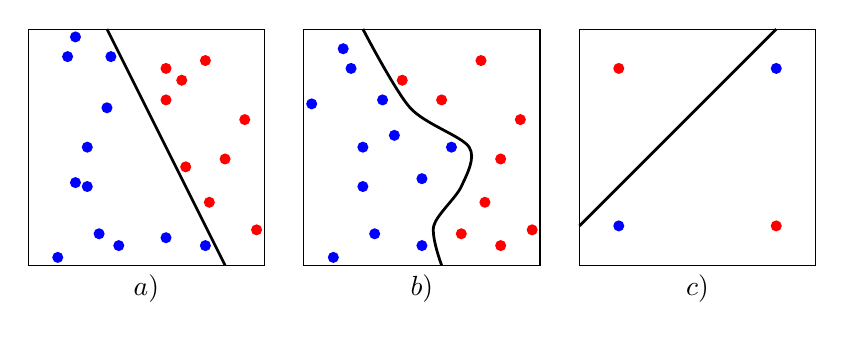
\begin{tikzpicture}[scale=0.5]
        % linearly separable box
        \draw (0,0) rectangle (6,6);
        \draw[text=black] (3,0) node[below] {$a)$};
        \draw[color=black,line width=1pt]
            (2,6) -- (5,0);

        % nonlinearly separable box
        \draw (7,0) rectangle (13,6);
        \draw[text=black] (10,0) node[below] {$b)$};
        \draw[color=black,line width=1pt] plot [smooth] coordinates {
            (8.5, 6) (9.7, 4) (11.2, 3) (11, 2) (10.3, 1) (10.5,0)};

        % XOR
        \draw (14,0) rectangle (20,6);
        \draw[text=black] (17,0) node[below] {$c)$};
        \draw[color=black,line width=1pt]
            (14,1) -- (19,6);

        \def\positive{{%
        % linear
        {.75, 0.2},
        {2.3, 0.5},
        {4.5, 0.5},
        {3.5, 0.7},
        {1.8, 0.8},
        {1.5, 2},
        {1.2, 2.1},
        {1.5, 3},
        {2, 4},
        {2.1, 5.3},
        {1, 5.3},
        {1.2, 5.8},
        % nonlinear
        {7.75, 0.2},
        {10, 0.5},
        {8.8, 0.8},
        {8.5, 2},
        {10, 2.2},
        {10.75, 3},
        {8.5, 3},
        {9.3, 3.3},
        {7.2, 4.1},
        {9, 4.2},
        {8.2, 5},
        {8, 5.5},
        % XOR
        {15, 1},
        {19, 5},
        }}

        % \draw positive dots
        \foreach \i in {0,...,25} {
          \pgfmathparse{\positive[\i][0]}\let \x \pgfmathresult;
          \pgfmathparse{\positive[\i][1]}\let \y \pgfmathresult;
          \fill[blue] (\x,\y) circle (4pt);
        }

        \def\negative{{%
        % linear
        {5.8, 0.9},
        {4.6, 1.6},
        {4, 2.5},
        {5, 2.7},
        {5.5, 3.7},
        {3.5, 4.2},
        {3.9, 4.7},
        {3.5, 5},
        {4.5, 5.2},
        % nonlinear
        {12, 0.5},
        {11, 0.8},
        {12.8, 0.9},
        {11.6, 1.6},
        {12, 2.7},
        {12.5, 3.7},
        {10.5, 4.2},
        {9.5, 4.7},
        {11.5, 5.2},
        % XOR
        {19, 1},
        {15, 5},
        }}

        % \draw negative dots
        \foreach \i in {0,...,19} {
          \pgfmathparse{\negative[\i][0]}\let \x \pgfmathresult;
          \pgfmathparse{\negative[\i][1]}\let \y \pgfmathresult;
          \fill[red] (\x,\y) circle (4pt);
        }
    \end{tikzpicture}
    \caption{a) A linearly separable problem. b) A nonlinearly separable
        problem. c) The XOR problem with a tentative solution that fails at
        separating the points of the space.\label{fig:XOR}}
\end{figure}

The excessive enthusiasm for the early successes of ANNs turned into strong
disappointment: even if~\cite{Minsky69} showed that an MLP could model the XOR
bitwise operation, it also pointed out that Rosenblatt's learning algorithm was
limited to single layered Perceptrons and could not autonomously learn how to
solve the problem. The expectation of an artificial intelligence that could
learn by itself to solve problems and interact with humans appeared suddenly
unrealistic and most of the research community lost interest in ANNs. The field
experienced a severe slow down and most of the fundings were cut.

After a decade known as the AI Winter, in 1982 John Hopfield presented a model
of the human memory that did not only give insights on how the brain works, but
was also useful in practical applications and had a sound and detail
mathematical grounding. At the same time at the US-Japan Joint Conference on
Cooperative/Competitive Neural Networks Japan announced a renewed effort in
building Neural Networks and the fear that the US might be left behind renewed
their effort on this topic.

The breakthrough that completely restored the interest in the field came in
1986, when~\cite{Rumelhart86b} rediscovered the backpropagation
algorithm~\citep{Linnainmaa70,Werbos74} that allowed to train ANNs composed by
multiple layers~(see \autoref{sec:backprop}). Since then ANNs have been
constantly focus of study and innovation and established the state of the art
in several domains.

% SCHMIDHUEBER
%In the new millennium, deep NNs have finally attracted wide-spread attention,
%mainly by outperforming alternative machine learning methods such as kernel
%machines in numerous important applications. In fact, since 2009, supervised
%deep NNs have won many official international pattern recognition competitions
%achieving the first superhuman visual pattern recognition results in limited
%domains.

\subsection{MultiLayer Perceptron}\label{sec:MLP}
\begin{figure}[h]
    \centering
    \begin{neuralnetwork} [nodespacing=7.5mm, layerspacing=23mm,
            maintitleheight=2.5em, layertitleheight=5em,
            height=3, toprow=true, nodesize=17pt,
            style={}, title={}, titlestyle={}]
        %%%%% Layers
        \inputlayer[count=2, bias=false, title=Input\\layer, text=\nodetextxi]
        \hiddenlayer[count=3, bias=true, title=Layer 1, text=\nodetexthi]
        {\setdefaultlinklabel{\wijllink}\linklayers}
        \hiddenlayer[count=5, bias=true, title=Layer 2, text=\nodetexthi]
        {\setdefaultlinklabel{\wijllink}\linklayers}
        \hiddenlayer[count=4, bias=true, title=Layer 3, text=\nodetexthi]
        {\setdefaultlinklabel{\wijllink}\linklayers}
        %\outputlayer[count=1, text=\nodetextsigma]
        %{\setdefaultlinklabel{\wijllink}\linklayers}
        %\redefinelayerspacing{20.5mm}
        %\outputlayer[count=1, text=\nodetextsigmoid]
        %\linklayers
        %\redefinelayerspacing{18.8mm}
        \outputlayer[count=1, text=\nodetexty]
        {\setdefaultlinklabel{\wijllink}\linklayers}
    \end{neuralnetwork}
    \centering
    \caption{\label{fig:MLP}A MultiLayer Perceptron. The sum and the
        nonlinearity nodes have been omitted for the sake of clarity.
    }
\end{figure}

Consider the network in~\autoref{fig:MLP}. As opposed to the Perceptron, the
MLP has multiple hidden layers, where each neuron of one hidden layer is
connected to all the neurons of the previous and next layer. Each connection
from a neuron $i$ to a neuron $j$ in layer $l$ is associated to a weight
$w_{ij}^{(l)}$. Similarly to the Perceptron case, each layer computes an affine
transformation, followed by a nonlinearity that is usually called
\emph{activation function}.
%that is usually different from the one proposed in the Perceptron paper.

The processing performed by the hierarchy of layers of the MLP is equivalent to
a composition of multiple functions

\begin{equation}\label{eq:fn_composition}
    y = h^{(L)}_{\theta} \circ
        h^{(L-1)}_{\theta} \circ
        \dots \circ
        h^{(1)}_{\theta}
\end{equation}

Each of these functions $h^{(l)}$ depends on some parameters - namely the
weights and bias of the layer, $W^{(l)}$ and $b^{(l)}$, as well as the choice
of activation function for the layer $a^{(l)}$. It is common to refer to the
parameters that fully characterize a layer as \emph{sufficient statistics},
usually denoted as $\theta$.

The MLP is not the only architecture used in ANNs. In \autoref{sec:cnn,sec:rnn}
two of the most used alternatives will be described. In general every layer of
an ANN will compute some activation based on its input and a nonlinearity, that
is usually different from the one proposed in the Perceptron paper. In the
following section, some of the most used activation functions will be
described.
%Generally, more complex activation functions than the one proposed in the
%Perceptron are being used. Here are some of the most frequently used ones.

\subsection{Activation functions}\label{sec:activations}
\begin{figure}[h]
    \centering
    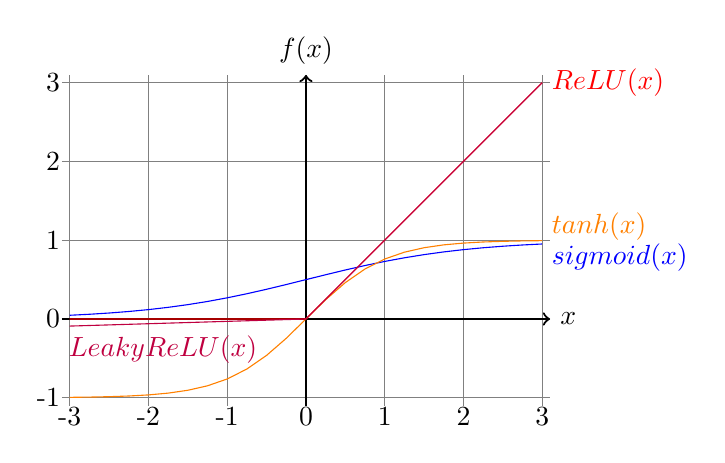
\begin{tikzpicture}[domain=-3:3]
        \draw[very thin,color=gray] (-3.1, -1.1) grid (3.1, 3.1);
        \foreach \x in {-3,-2,-1,0,1,2,3}
            \node[anchor=north] at (\x,-1) {\x};
        \foreach \y in {-1,0,1,2,3}
            \node[anchor=east] at (-3,\y) {\y};
        % axes
        \draw[->,thick] (-3.1, 0) -- (3.1, 0) node[right] {$x$};
        \draw[->,thick] (0, -1.1) -- (0, 3.1) node[above] {$f(x)$};

        % activations
        \draw[color=blue] plot (\x, { 1/(1+exp(-1 * \x)) })
            node[right,yshift=-0.5em] {$sigmoid(x)$};
        %\draw[color=yellow] plot (\x, { 1/(1+exp(-.5 * \x)) })
        %    node[right] {$f(x) = sigmoid(x), beta=.5$};
        \draw[color=orange] plot (\x, { ( 1 - exp(-2*\x) ) / ( 1 + exp(-2*\x) ) })
            node[right,yshift=0.5em] {$tanh(x)$};
        \draw[color=red] plot (\x, { max(0, \x) })
            node[right] {$ReLU(x)$};
        \draw[color=purple] plot (\x, { max(0.03 * \x, \x) })
            node[above, xshift=-13.7em,yshift=-10.5em] {$Leaky ReLU(x)$};
    \end{tikzpicture}
    \caption{Some of the most common activation functions: sigmoid, tanh, ReLU
        and Leaky ReLU\label{fig:activations}}
\end{figure}

The activation function is one of the most important component of an ANN. As
explained in the previous sections, to tackle nonlinearly separable problems it
is imperative to map the input into a space that is linearly separable. The
activation function does this by performing an \emph{element-wise nonlinear
transformation} of the pre-activation that comes from the affine
transformation.

The affine transformation and the nonlinearity work together in a very tight
interaction: the latter is fixed and does not evolve during training, but
is a powerful transformation; the former instead, is determined by the weights
that are learned during training and exploits the latter to separate the
incoming activation so that they are easier to separate.

In addition to this, it is interesting to point out that if there was no
activation function, the composition of multiple affine transformation would
reduce to being an affine transformation, and the MLP would go back to being a
Perceptron.

\subsubsection{logistic}\label{sec:logistic}
The logistic
sigmoid $\frac{1}{1+exp(-x)}$
tanh $\frac{1}{1+exp(-x)}$
relu $\frac{1}{1+exp(-x)}$
sigmoid $\frac{1}{1+exp(-x)}$


\subsection{Backpropagation}\label{sec:backprop}
The learning rule introduced with Perceptrons does not allow to train models
with multiple layers (i.e. with \emph{hidden} layers), such as the one depicted
in~\autoref{fig:MLP}.

This is not possible due to the fact that to compute the variation of the
weights of a layer with~\autoref{eq:perceptron_lr} it is necessary to know the
correct value of its output, which is known only for the last layer. To address
this apparently insurmountable obstacle it suffices to notice that the
computation performed by the activation function is a nonlinear but
differentiable function of the inputs. This allows for computing the
partial derivatives of the error, i.e. the difference between the desired
output and the actual one, w.r.t. the weights of the network. In other words,
it is possible to use calculus to determine the amount by which each neuron of
the last layer contributed to causing the error, and then further split the
responsibility of each of them among the ones of the preceding layer. This way
the error can be \emph{backpropagated} through the layers of the network,
assigning to each weight its amount of blame. This information can be used by
an \emph{optimization algorithm} to iteratively change the weights to minimize
the error.

The backpropagation algorithm has some resemblance with the learning rule of
the Perceptron~(\autoref{eq:perceptron_lr}). The main idea in that case was
to modify each weight of the network by a factor proportional to the error $E =
\hat y - y$ and to the input. Even if in MLP it is usually common to consider
other kinds of errors, such as the mean squared error (MSE) $E_{MSE} =
\frac{1}{n} \sum_{i=0}^n(\hat y_i - y_i)^2$, the same concept applies: the
learning procedure tries to modify the weights in order to minimize the error.

The rest of this chapter will focus on two very common kinds of ANNs
respectively characterized by a feedforward and feedback connectivity pattern,
namely Convolutional Neural Networks and Recurrent Neural Networks.


%================================== SECTION ==================================
\section{Convolutional networks}\label{sec:convnets}

Deep convolutional neural networks (CNNs) have been at the heart of spectacular
advances in deep learning. Although CNNs have been used as early as the nineties
to solve character recognition tasks \citep{le1997reading}, their current
widespread application is due to much more recent work, when a deep CNN was used
to beat state-of-the-art in the ImageNet image classification challenge
\citep{krizhevsky2012imagenet}.

Convolutional neural networks therefore constitute a very useful tool for
machine learning practitioners.
However, learning to use CNNs for the first time
is generally an intimidating experience. A convolutional layer's output shape is
affected by the shape of its input as well as the choice of kernel shape, zero
padding and strides, and the relationship between these properties is not
trivial to infer. This contrasts with fully-connected layers, whose output size
is independent of the input size. Additionally, CNNs also usually feature a {\em
pooling\/} stage, adding yet another level of complexity with respect to
fully-connected networks.  Finally, so-called transposed convolutional layers
(also known as fractionally strided convolutional layers) have been employed in
more and more work as of late \citep{zeiler2011adaptive,zeiler2014visualizing,
long2015fully,radford2015unsupervised,visin15,im2016generating}, and their
relationship with convolutional layers has been explained with various degrees
of clarity.

For an in-depth treatment of the subject, see Chapter 9 of the Deep Learning
textbook \citep{Goodfellow-et-al-2016-Book}.

\section{Discrete convolutions}

The bread and butter of neural networks is \emph{affine transformations}: a
vector is received as input and is multiplied with a matrix to produce an
output (to which a bias vector is usually added before passing the result
through a nonlinearity). This is applicable to any type of input, be it an
image, a sound clip or an unordered collection of features: whatever their
dimensionality, their representation can always be flattened into a vector
before the transformation.

Images, sound clips and many other similar kinds of data have an intrinsic
structure. More formally, they share these important properties:

\begin{itemize}
    \item They are stored as multi-dimensional arrays.
    \item They feature one or more axes for which ordering matters (e.g., width
        and height axes for an image, time axis for a sound clip).
    \item One axis, called the channel axis, is used to access different views
        of the data (e.g., the red, green and blue channels of a color image, or
        the left and right channels of a stereo audio track).
\end{itemize}

These properties are not exploited when an affine transformation is applied; in
fact, all the axes are treated in the same way and the topological information
is not taken into account. Still, taking advantage of the implicit structure of
the data may prove very handy in solving some tasks, like computer vision and
speech recognition, and in these cases it would be best to preserve it. This is
where discrete convolutions come into play.

A discrete convolution is a linear transformation that preserves this notion of
ordering. It is sparse (only a few input units contribute to a given output
unit) and reuses parameters (the same weights are applied to multiple locations
in the input).

\autoref{fig:numerical_no_padding_no_strides} provides an example of a discrete
convolution. The light blue grid is called the {\em input feature map}. To keep
the drawing simple, a single input feature map is represented, but it is not
uncommon to have multiple feature maps stacked one onto another.\footnote{%
    An example of this is what was referred to earlier as {\em channels\/} for
    images and sound clips.}
A {\em kernel\/} (shaded area) of value

\begin{figure}[H]
    \centering
    \begin{tikzpicture}[scale=.4,every node/.style={minimum size=1cm}, on grid]
            \draw[fill=base02,opacity=0.4] (0,0) rectangle (3,3);
            \draw[draw=base03,thick] (0,0) grid (3,3);
            \node (00) at (0.5,2.5) {\tiny 0};
            \node (01) at (1.5,2.5) {\tiny 1};
            \node (02) at (2.5,2.5) {\tiny 2};
            \node (10) at (0.5,1.5) {\tiny 2};
            \node (11) at (1.5,1.5) {\tiny 2};
            \node (12) at (2.5,1.5) {\tiny 0};
            \node (20) at (0.5,0.5) {\tiny 0};
            \node (21) at (1.5,0.5) {\tiny 1};
            \node (22) at (2.5,0.5) {\tiny 2};
    \end{tikzpicture}
\end{figure}

\begin{figure}[p]
    \centering
    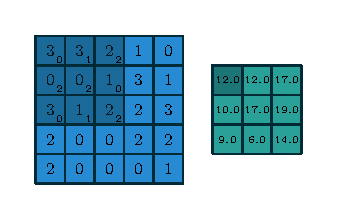
\includegraphics[width=0.32\textwidth]{pdf/numerical_no_padding_no_strides_00.pdf}
    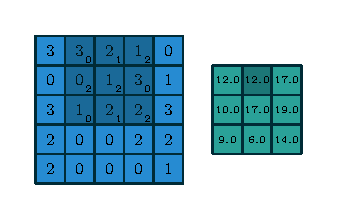
\includegraphics[width=0.32\textwidth]{pdf/numerical_no_padding_no_strides_01.pdf}
    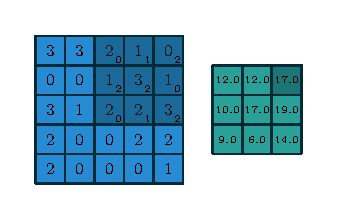
\includegraphics[width=0.32\textwidth]{pdf/numerical_no_padding_no_strides_02.pdf}
    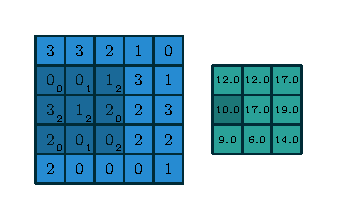
\includegraphics[width=0.32\textwidth]{pdf/numerical_no_padding_no_strides_03.pdf}
    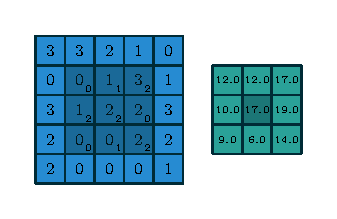
\includegraphics[width=0.32\textwidth]{pdf/numerical_no_padding_no_strides_04.pdf}
    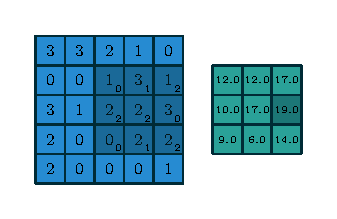
\includegraphics[width=0.32\textwidth]{pdf/numerical_no_padding_no_strides_05.pdf}
    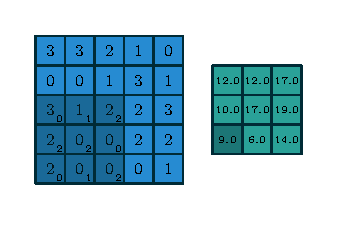
\includegraphics[width=0.32\textwidth]{pdf/numerical_no_padding_no_strides_06.pdf}
    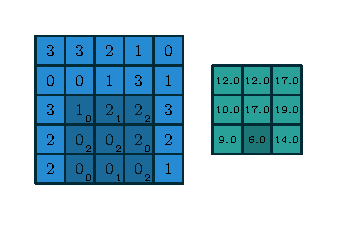
\includegraphics[width=0.32\textwidth]{pdf/numerical_no_padding_no_strides_07.pdf}
    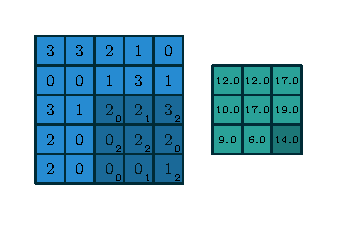
\includegraphics[width=0.32\textwidth]{pdf/numerical_no_padding_no_strides_08.pdf}
    \caption{\label{fig:numerical_no_padding_no_strides} Computing the output
        values of a discrete convolution.}
\end{figure}

\begin{figure}[p]
    \centering
    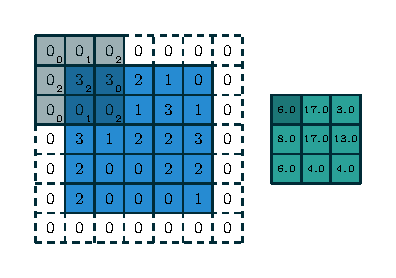
\includegraphics[width=0.32\textwidth]{pdf/numerical_padding_strides_00.pdf}
    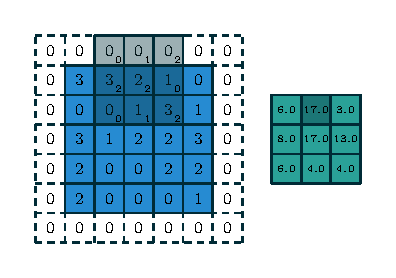
\includegraphics[width=0.32\textwidth]{pdf/numerical_padding_strides_01.pdf}
    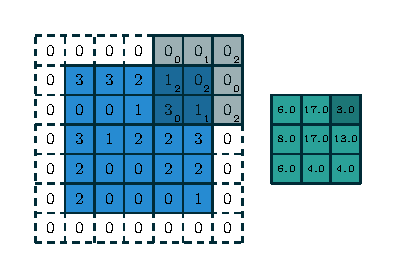
\includegraphics[width=0.32\textwidth]{pdf/numerical_padding_strides_02.pdf}
    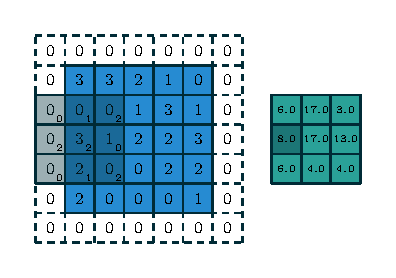
\includegraphics[width=0.32\textwidth]{pdf/numerical_padding_strides_03.pdf}
    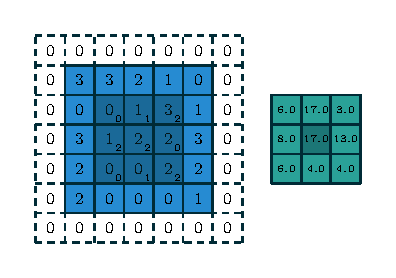
\includegraphics[width=0.32\textwidth]{pdf/numerical_padding_strides_04.pdf}
    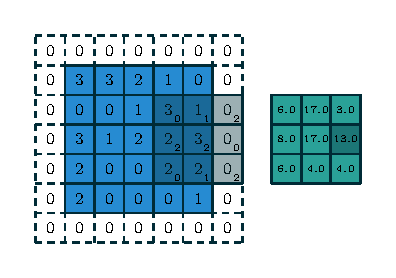
\includegraphics[width=0.32\textwidth]{pdf/numerical_padding_strides_05.pdf}
    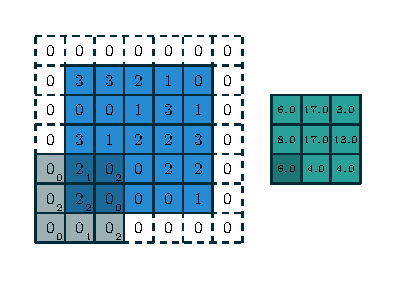
\includegraphics[width=0.32\textwidth]{pdf/numerical_padding_strides_06.pdf}
    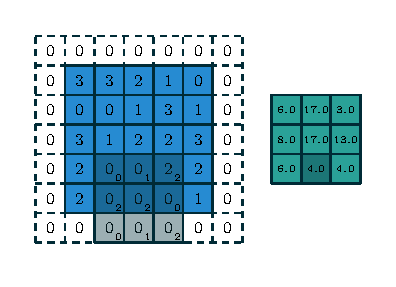
\includegraphics[width=0.32\textwidth]{pdf/numerical_padding_strides_07.pdf}
    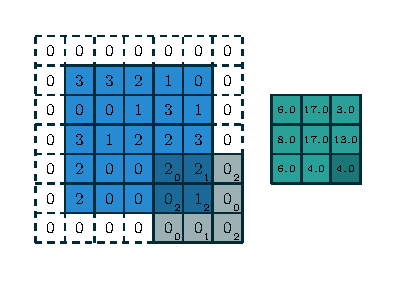
\includegraphics[width=0.32\textwidth]{pdf/numerical_padding_strides_08.pdf}
    \caption{\label{fig:numerical_padding_strides} Computing the output values
        of a discrete convolution for $N = 2$, $i_1 = i_2 = 5$, $k_1 = k_2 = 3$,
        $s_1 = s_2 = 2$, and $p_1 = p_2 = 1$.}
\end{figure}

\noindent slides across the input feature map. At each location, the product
between each element of the kernel and the input element it overlaps is computed
and the results are summed up to obtain the output in the current location. The
procedure can be repeated using different kernels to form as many output feature
maps as desired (\autoref{fig:full_picture}). The final outputs of this procedure
are called {\em output feature maps}.\footnote{%
    While there is a distinction between convolution and cross-correlation from
    a signal processing perspective, the two become interchangeable when the
    kernel is learned. For the sake of simplicity and to stay consistent with
    most of the machine learning literature, the term {\em convolution\/}
    will be used in this guide.}
If there are multiple input feature maps, the kernel will have to be
3-dimensional -- or, equivalently each one of the feature maps will be
convolved with a distinct kernel -- and the resulting feature maps will
be summed up elementwise to produce the output feature map.

The convolution depicted in \autoref{fig:numerical_no_padding_no_strides} is an
instance of a 2-D convolution, but it can be generalized to N-D convolutions.
For instance, in a 3-D convolution, the kernel would be a {\em cuboid\/} and
would slide across the height, width and depth of the input feature map.

The collection of kernels defining a discrete convolution has a shape
corresponding to some permutation of $(n, m, k_1, \ldots, k_N)$, where

\begin{equation*}
\begin{split}
    n &\equiv \text{number of output feature maps},\\
    m &\equiv \text{number of input feature maps},\\
    k_j &\equiv \text{kernel size along axis $j$}.
\end{split}
\end{equation*}

The following properties affect the output size $o_j$ of a convolutional layer
along axis $j$:

\begin{itemize}
    \item $i_j$: input size along axis $j$,
    \item $k_j$: kernel size along axis $j$,
    \item $s_j$: stride (distance between two consecutive positions of the
        kernel) along axis $j$,
    \item $p_j$: zero padding (number of zeros concatenated at the beginning and
        at the end of an axis) along axis $j$.
\end{itemize}

\noindent For instance, \autoref{fig:numerical_padding_strides} shows a $3
\times 3$ kernel applied to a $5 \times 5$ input padded with a $1 \times 1$
border of zeros using $2 \times 2$ strides.

Note that strides constitute a form of \emph{subsampling}. As an alternative to
being interpreted as a measure of how much the kernel is translated, strides
can also be viewed as how much of the output is retained. For instance, moving
the kernel by hops of two is equivalent to moving the kernel by hops of one but
retaining only odd output elements (\autoref{fig:strides_subsampling}).

\begin{figure}[p]
    \centering
    \begin{tikzpicture}[scale=.35,every node/.style={minimum size=1cm}, on grid]
        \begin{scope}[xshift=0cm,yshift=0cm]
            \begin{scope}[xshift=0cm,yshift=0cm]
                \draw[draw=base03,fill=violet,thick]
                    (0,0) grid (5,5) rectangle (0,0);
            \end{scope}
            \begin{scope}[xshift=0.5cm,yshift=0.5cm]
                \draw[draw=base03,fill=blue,thick]
                    (0,0) grid (5,5) rectangle (0,0);
            \end{scope}
        \end{scope}
        \foreach \x in {-10,1,11} {%
            \begin{scope}[xshift=\x cm,yshift=10cm]
                \begin{scope}[xshift=0cm,yshift=0cm]
                    \draw[draw=base03,fill=violet,thick]
                        (0,0) grid (3,3) rectangle (0,0);
                \end{scope}
                \begin{scope}[xshift=0.5cm,yshift=0.5cm]
                    \draw[draw=base03,fill=blue,thick]
                        (0,0) grid (3,3) rectangle (0,0);
                \end{scope}
            \end{scope}
            \begin{scope}[xshift=\x cm,yshift=20cm]\begin{scope}[xshift=0.5cm]
                \draw[draw=base03,fill=cyan,thick]
                    (0,0) grid (3,3) rectangle (0,0);
            \end{scope}\end{scope}
        }
        \begin{scope}[xshift=1cm,yshift=30cm]
            \foreach \s in {0.0,0.5,1.0} {%
                \begin{scope}[xshift=\s cm,yshift=\s cm]
                    \draw[draw=base03,fill=cyan,thick]
                        (0,0) grid (3,3) rectangle (0,0);
                \end{scope}
            }
        \end{scope}
        \draw[->, thick] (-0.5,2.5) to (-8.5,9.5);
        \draw[->, thick] (3,6) to (3,9.5);
        \draw[->, thick] (6,3.5) to (12.5,9.5);
        \draw[thick]  (-8,14.5) to (-8,16);
        \draw[->, thick]  (-8,18) to (-8,19.5);
        \node[thick] (p1) at (-8,17) {$+$};
        \draw[thick]  (3,14.5) to (3,16);
        \draw[->, thick]  (3,18) to (3,19.5);
        \node[thick] (p2) at (3,17) {$+$};
        \draw[thick]  (13,14.5) to (13,16);
        \draw[->, thick]  (13,18) to (13,19.5);
        \node[thick] (p3) at (13,17) {$+$};
        \draw[->, thick]  (-8,23.5) to (2,29.5);
        \draw[->, thick]  (3,23.5) to (2.5,29.5);
        \draw[->, thick]  (13,23.5) to (3,29.5);
    \end{tikzpicture}
    \caption{\label{fig:full_picture} A convolution mapping from two input
        feature maps to three output feature maps using a $3 \times 2 \times 3
        \times 3$ collection of kernels $\mathbf{w}$. In the left pathway, input
        feature map 1 is convolved with kernel $\mathbf{w}_{1,1}$ and input
        feature map 2 is convolved with kernel $\mathbf{w}_{1,2}$, and the
        results are summed together elementwise to form the first output feature
        map. The same is repeated for the middle and right pathways to form the
        second and third feature maps, and all three output feature maps are
        grouped together to form the output.}
\end{figure}

\begin{figure}[p]
    \centering
    \begin{tikzpicture}[scale=.35,every node/.style={minimum size=1cm}, on grid]
        \begin{scope}[xshift=0,yshift=0cm]
            \begin{scope}[xshift=0cm,yshift=0cm]
                \draw[draw=base03,fill=blue,thick] (0,0) grid (5,5) rectangle (0,0);
                \draw[fill=base02, opacity=0.4] (0,2) rectangle (3,5);
            \end{scope}
            \begin{scope}[xshift=7cm,yshift=1.5cm]
                \draw[draw=base03,fill=cyan,thick] (0,0) grid (2,2) rectangle (0,0);
            \end{scope}
        \end{scope}
        \draw[draw=base03, ->, thick] (2.6,3.5) to  (4.5,3.5);
        \draw[draw=base03, ->, thick] (1.5,2.4) to (1.5,0.5);
        \draw[draw=base03, ->, thick] (5.25, 2.5) to (6.75, 2.5);
        \begin{scope}[xshift=12cm,yshift=0cm]
            \begin{scope}[xshift=0cm,yshift=0cm]
                \draw[draw=base03,fill=blue,thick] (0,0) grid (5,5) rectangle (0,0);
                \draw[fill=base02, opacity=0.4] (0,2) rectangle (3,5);
            \end{scope}
            \begin{scope}[xshift=7cm,yshift=1cm]
                \draw[draw=base03,fill=cyan,thick] (0,0) grid (3,3) rectangle (0,0);
                \draw[draw=base03] (1,0) -- (2,1) -- (2,0) -- (1,1);
                \draw[draw=base03] (0,1) -- (1,2) -- (1,1) -- (0,2);
                \draw[draw=base03] (1,1) -- (2,2) -- (2,1) -- (1,2);
                \draw[draw=base03] (2,1) -- (3,2) -- (3,1) -- (2,2);
                \draw[draw=base03] (1,2) -- (2,3) -- (2,2) -- (1,3);
            \end{scope}
            \begin{scope}[xshift=12cm,yshift=1.5cm]
                \draw[draw=base03,fill=cyan,thick] (0,0) grid (2,2) rectangle (0,0);
            \end{scope}
        \end{scope}
        \draw[draw=base03, ->, thick] (14.6,3.5) to  (15.5,3.5);
        \draw[draw=base03, ->, thick] (15.6,3.5) to  (16.5,3.5);
        \draw[draw=base03, ->, thick] (13.5,2.4) to (13.5,1.5);
        \draw[draw=base03, ->, thick] (13.5,1.4) to (13.5,0.5);
        \draw[draw=base03, ->, thick] (17.25, 2.5) to (18.75, 2.5);
        \draw[draw=base03, ->, thick] (22.25, 2.5) to (23.75, 2.5);
    \end{tikzpicture}
    \caption{\label{fig:strides_subsampling} An alternative way of viewing
        strides. Instead of translating the $3 \times 3$ kernel by increments of
        $s = 2$ (left), the kernel is translated by increments of $1$ and only
        one in $s = 2$ output elements is retained (right).}
\end{figure}

\section{Pooling}

In addition to discrete convolutions themselves, {\em pooling\/} operations
make up another important building block in CNNs. Pooling operations reduce
the size of feature maps by using some function to summarize subregions, such
as taking the average or the maximum value.

Pooling works by sliding a window across the input and feeding the content of
the window to a {\em pooling function}. In some sense, pooling works very much
like a discrete convolution, but replaces the linear combination described by
the kernel with some other function. \autoref{fig:numerical_average_pooling}
provides an example for average pooling, and \autoref{fig:numerical_max_pooling}
does the same for max pooling.

The following properties affect the output size $o_j$ of a pooling layer
along axis $j$:

\begin{itemize}
    \item $i_j$: input size along axis $j$,
    \item $k_j$: pooling window size along axis $j$,
    \item $s_j$: stride (distance between two consecutive positions of the
        pooling window) along axis $j$.
\end{itemize}

\begin{figure}[p]
    \centering
    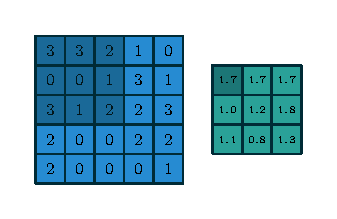
\includegraphics[width=0.32\textwidth]{pdf/numerical_average_pooling_00.pdf}
    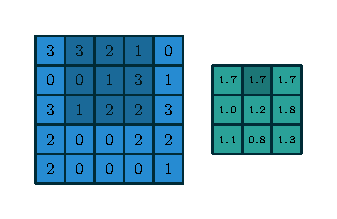
\includegraphics[width=0.32\textwidth]{pdf/numerical_average_pooling_01.pdf}
    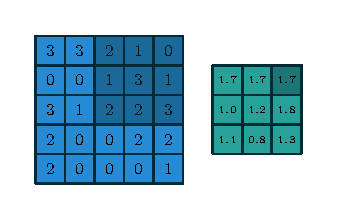
\includegraphics[width=0.32\textwidth]{pdf/numerical_average_pooling_02.pdf}
    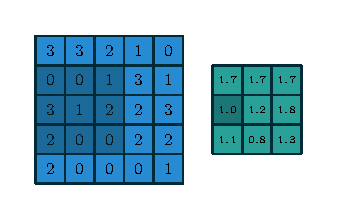
\includegraphics[width=0.32\textwidth]{pdf/numerical_average_pooling_03.pdf}
    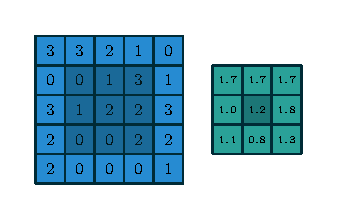
\includegraphics[width=0.32\textwidth]{pdf/numerical_average_pooling_04.pdf}
    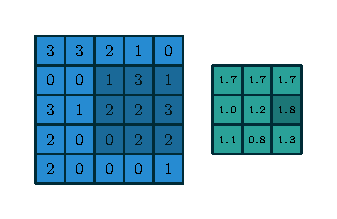
\includegraphics[width=0.32\textwidth]{pdf/numerical_average_pooling_05.pdf}
    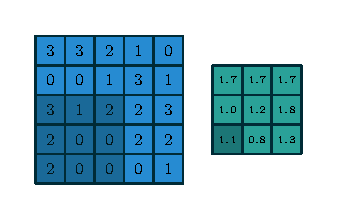
\includegraphics[width=0.32\textwidth]{pdf/numerical_average_pooling_06.pdf}
    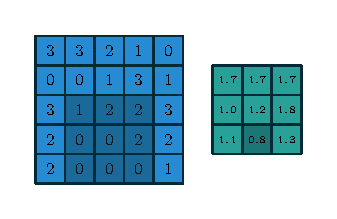
\includegraphics[width=0.32\textwidth]{pdf/numerical_average_pooling_07.pdf}
    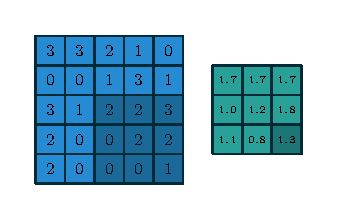
\includegraphics[width=0.32\textwidth]{pdf/numerical_average_pooling_08.pdf}
    \caption{\label{fig:numerical_average_pooling} Computing the output values
        of a $3 \times 3$ average pooling operation on a $5 \times 5$ input
        using $1 \times 1$ strides.}
\end{figure}

\begin{figure}[p]
    \centering
    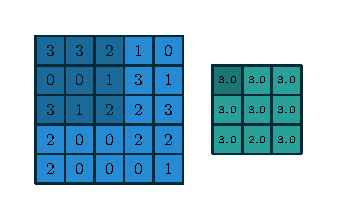
\includegraphics[width=0.32\textwidth]{pdf/numerical_max_pooling_00.pdf}
    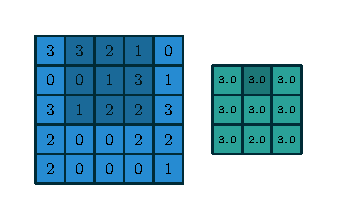
\includegraphics[width=0.32\textwidth]{pdf/numerical_max_pooling_01.pdf}
    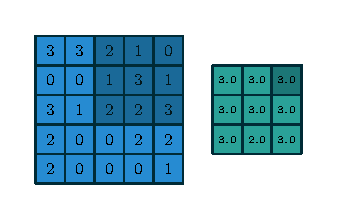
\includegraphics[width=0.32\textwidth]{pdf/numerical_max_pooling_02.pdf}
    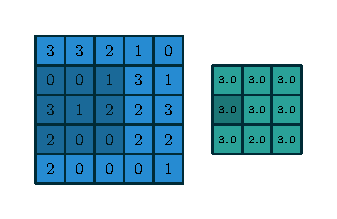
\includegraphics[width=0.32\textwidth]{pdf/numerical_max_pooling_03.pdf}
    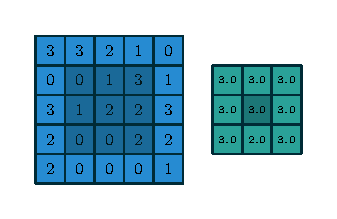
\includegraphics[width=0.32\textwidth]{pdf/numerical_max_pooling_04.pdf}
    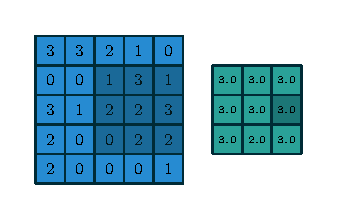
\includegraphics[width=0.32\textwidth]{pdf/numerical_max_pooling_05.pdf}
    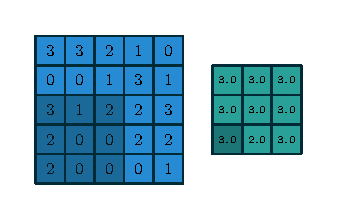
\includegraphics[width=0.32\textwidth]{pdf/numerical_max_pooling_06.pdf}
    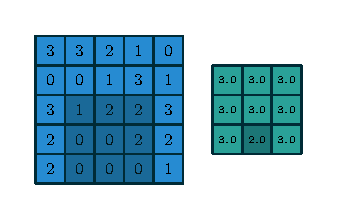
\includegraphics[width=0.32\textwidth]{pdf/numerical_max_pooling_07.pdf}
    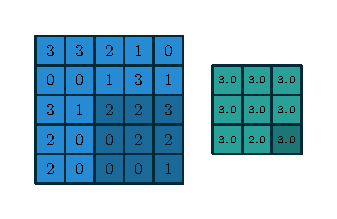
\includegraphics[width=0.32\textwidth]{pdf/numerical_max_pooling_08.pdf}
    \caption{\label{fig:numerical_max_pooling} Computing the output values of a
        $3 \times 3$ max pooling operation on a $5 \times 5$ input using $1
        \times 1$ strides.}
\end{figure}

\chapter{Convolution arithmetic}

The analysis of the relationship between convolutional layer properties is eased
by the fact that they don't interact across axes, i.e., the choice of kernel
size, stride and zero padding along axis $j$ only affects the output size of
axis $j$. Because of that, this chapter will focus on the following simplified
setting:

\begin{itemize}
    \item 2-D discrete convolutions ($N = 2$),
    \item square inputs ($i_1 = i_2 = i$),
    \item square kernel size ($k_1 = k_2 = k$),
    \item same strides along both axes ($s_1 = s_2 = s$),
    \item same zero padding along both axes ($p_1 = p_2 = p$).
\end{itemize}

This facilitates the analysis and the visualization, but keep in mind that the
results outlined here also generalize to the N-D and non-square cases.

\section{No zero padding, unit strides}

The simplest case to analyze is when the kernel just slides across every
position of the input (i.e., $s = 1$ and $p = 0$).
\autoref{fig:no_padding_no_strides} provides an example for $i = 4$ and $k =
3$.

One way of defining the output size in this case is by the number of possible
placements of the kernel on the input. Let's consider the width axis: the kernel
starts on the leftmost part of the input feature map and slides by steps of one
until it touches the right side of the input. The size of the output will be
equal to the number of steps made, plus one, accounting for the initial position
of the kernel (\autoref{fig:no_padding_no_strides_explained}). The same logic
applies for the height axis.

More formally, the following relationship can be inferred:

\begin{relationship}\label{rel:no_padding_no_strides}
For any $i$ and $k$, and for $s = 1$ and $p = 0$,
\begin{equation*}
    o = (i - k) + 1.
\end{equation*}
\end{relationship}

\begin{figure}[p]
    \centering
    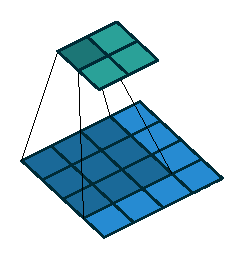
\includegraphics[width=0.24\textwidth]{pdf/no_padding_no_strides_00.pdf}
    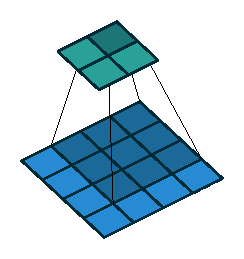
\includegraphics[width=0.24\textwidth]{pdf/no_padding_no_strides_01.pdf}
    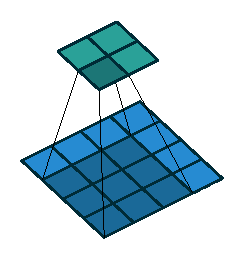
\includegraphics[width=0.24\textwidth]{pdf/no_padding_no_strides_02.pdf}
    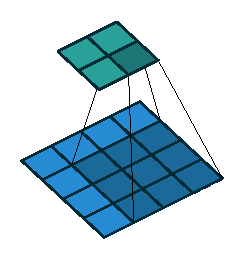
\includegraphics[width=0.24\textwidth]{pdf/no_padding_no_strides_03.pdf}
    \caption{\label{fig:no_padding_no_strides} (No padding, unit strides)
        Convolving a $3 \times 3$ kernel over a $4 \times 4$ input using unit
        strides (i.e., $i = 4$, $k = 3$, $s = 1$ and $p = 0$).}
\end{figure}

\begin{figure}[p]
    \centering
    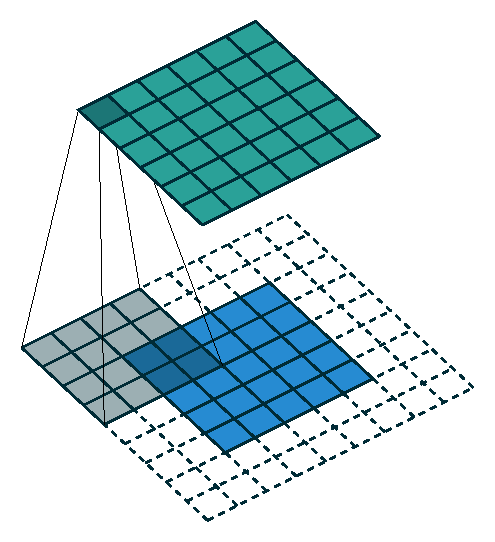
\includegraphics[width=0.24\textwidth]{pdf/arbitrary_padding_no_strides_00.pdf}
    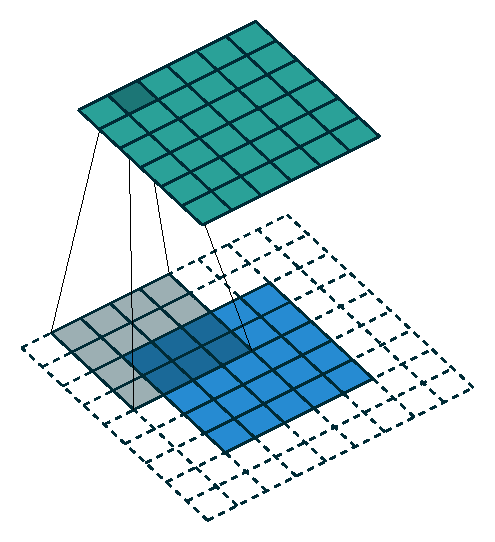
\includegraphics[width=0.24\textwidth]{pdf/arbitrary_padding_no_strides_01.pdf}
    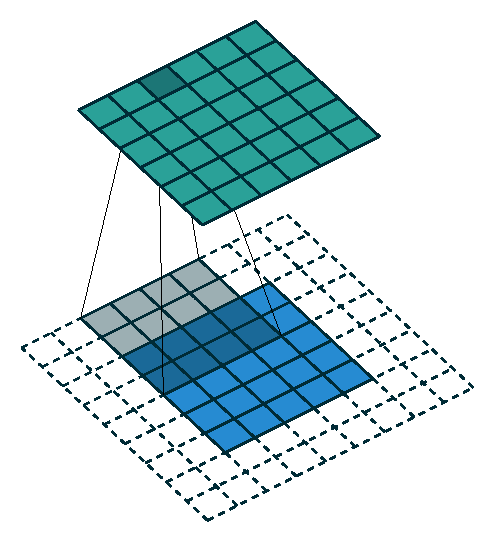
\includegraphics[width=0.24\textwidth]{pdf/arbitrary_padding_no_strides_02.pdf}
    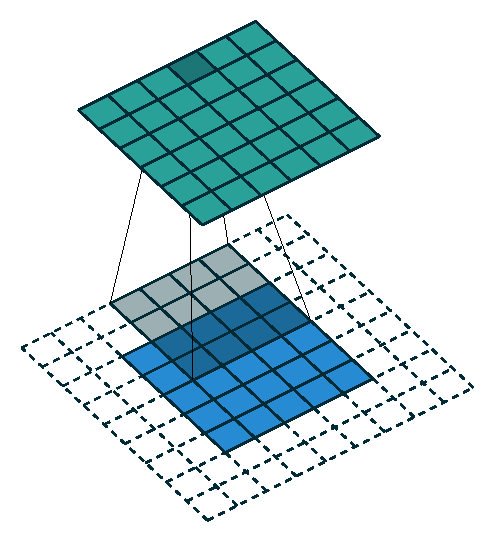
\includegraphics[width=0.24\textwidth]{pdf/arbitrary_padding_no_strides_03.pdf}
    \caption{\label{fig:arbitrary_padding_no_strides} (Arbitrary padding, unit
        strides) Convolving a $4 \times 4$ kernel over a $5 \times 5$ input
        padded with a $2 \times 2$ border of zeros using unit strides (i.e.,
        $i = 5$, $k = 4$, $s = 1$ and $p = 2$).}
\end{figure}

\begin{figure}[p]
    \centering
    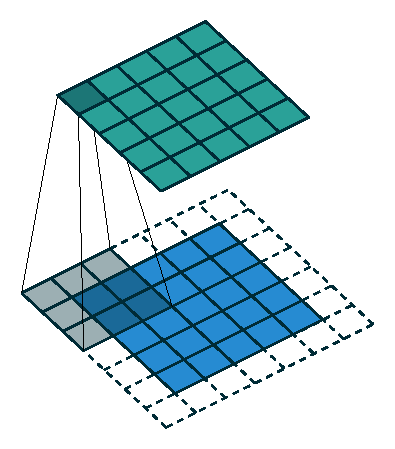
\includegraphics[width=0.24\textwidth]{pdf/same_padding_no_strides_00.pdf}
    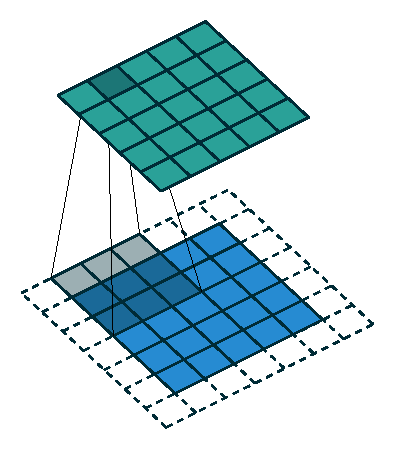
\includegraphics[width=0.24\textwidth]{pdf/same_padding_no_strides_01.pdf}
    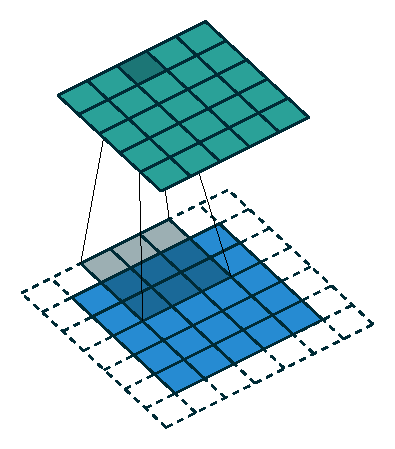
\includegraphics[width=0.24\textwidth]{pdf/same_padding_no_strides_02.pdf}
    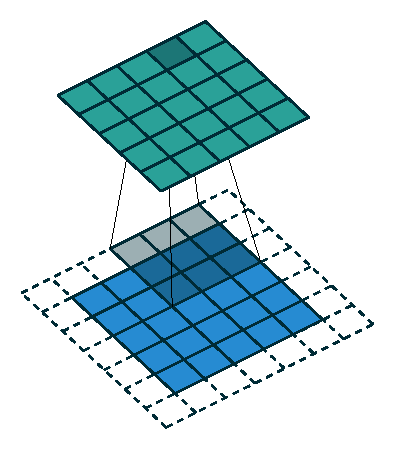
\includegraphics[width=0.24\textwidth]{pdf/same_padding_no_strides_03.pdf}
    \caption{\label{fig:same_padding_no_strides} (Half padding, unit strides)
        Convolving a $3 \times 3$ kernel over a $5 \times 5$ input using half
        padding and unit strides (i.e., $i = 5$, $k = 3$, $s = 1$ and $p = 1$).}
\end{figure}

\begin{figure}[p]
    \centering
    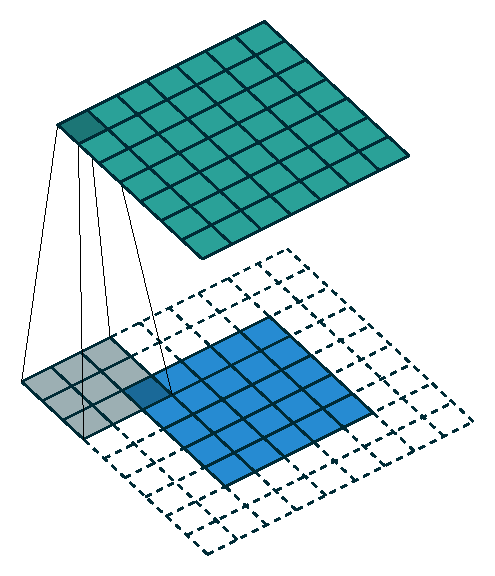
\includegraphics[width=0.24\textwidth]{pdf/full_padding_no_strides_00.pdf}
    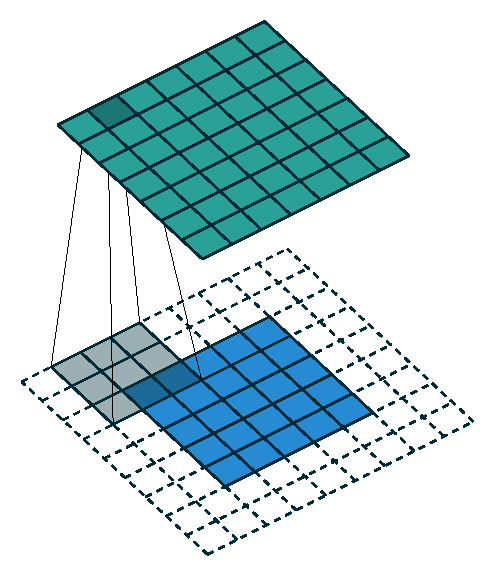
\includegraphics[width=0.24\textwidth]{pdf/full_padding_no_strides_01.pdf}
    \includegraphics[width=0.24\textwidth]{pdf/full_padding_no_strides_02.pdf}
    \includegraphics[width=0.24\textwidth]{pdf/full_padding_no_strides_03.pdf}
    \caption{\label{fig:full_padding_no_strides} (Full padding, unit strides)
        Convolving a $3 \times 3$ kernel over a $5 \times 5$ input using full
        padding and unit strides (i.e., $i = 5$, $k = 3$, $s = 1$ and $p = 2$).}
\end{figure}

\section{Zero padding, unit strides}

To factor in zero padding (i.e., only restricting to $s = 1$), let's consider
its effect on the effective input size: padding with $p$ zeros changes the
effective input size from $i$ to $i + 2p$. In the general case,
\autoref{rel:no_padding_no_strides} can then be used to infer the following
relationship:

\begin{relationship}\label{rel:arbitrary_padding_no_strides}
For any $i$, $k$ and $p$, and for $s = 1$,
\begin{equation*}
    o = (i - k) + 2p + 1.
\end{equation*}
\end{relationship}

\noindent \autoref{fig:arbitrary_padding_no_strides} provides an example for $i
= 5$, $k = 4$ and $p = 2$.

In practice, two specific instances of zero padding are used quite extensively
because of their respective properties. Let's discuss them in more detail.

\subsection{Half (same) padding}

Having the output size be the same as the input size (i.e., $o = i$) can be a
desirable property:

\begin{relationship}\label{rel:same_padding_no_strides}
For any $i$ and for $k$ odd ($k = 2n + 1, \quad n \in \mathbb{N}$), $s = 1$ and
$p = \lfloor k / 2 \rfloor = n$,
\begin{equation*}
\begin{split}
    o &= i + 2 \lfloor k / 2 \rfloor - (k - 1) \\
      &= i + 2n - 2n \\
      &= i.
\end{split}
\end{equation*}
\end{relationship}

\noindent This is sometimes referred to as {\em half\/} (or {\em same\/})
padding. \autoref{fig:same_padding_no_strides} provides an example for
$i = 5$, $k = 3$ and (therefore) $p = 1$.

\subsection{Full padding}

While convolving a kernel generally {\em decreases\/} the output size with
respect to the input size, sometimes the opposite is required. This can be
achieved with proper zero padding:

\begin{relationship}\label{rel:full_padding_no_strides}
For any $i$ and $k$, and for $p = k - 1$ and $s = 1$,
\begin{equation*}
\begin{split}
    o &= i + 2(k - 1) - (k - 1) \\
      &= i + (k - 1).
\end{split}
\end{equation*}
\end{relationship}

\noindent This is sometimes referred to as {\em full\/} padding, because in this
setting every possible partial or complete superimposition of the kernel on the
input feature map is taken into account. \autoref{fig:full_padding_no_strides}
provides an example for $i = 5$, $k = 3$ and (therefore) $p = 2$.

\section{No zero padding, non-unit strides}

All relationships derived so far only apply for unit-strided convolutions.
Incorporating non unitary strides requires another inference leap. To
facilitate the analysis, let's momentarily ignore zero padding (i.e., $s > 1$
and $p = 0$). \autoref{fig:no_padding_strides} provides an example for $i =
5$, $k = 3$ and $s = 2$.

Once again, the output size can be defined in terms of the number of possible
placements of the kernel on the input. Let's consider the width axis: the
kernel starts as usual on the leftmost part of the input, but this time it
slides by steps of size $s$ until it touches the right side of the input. The
size of the output is again equal to the number of steps made, plus one,
accounting for the initial position of the kernel
(\autoref{fig:no_padding_strides_explained}). The same logic applies for the
height axis.

From this, the following relationship can be inferred:

\begin{relationship}\label{rel:no_padding_strides}
For any $i$, $k$ and $s$, and for $p = 0$,
\begin{equation*}
    o = \left\lfloor \frac{i - k}{s} \right\rfloor + 1.
\end{equation*}
\end{relationship}

\noindent The floor function accounts for the fact that sometimes the last
possible step does {\em not\/} coincide with the kernel reaching the end of the
input, i.e., some input units are left out (see
\autoref{fig:padding_strides_odd} for an example of such a case).

\section{Zero padding, non-unit strides}

The most general case (convolving over a zero padded input using non-unit
strides) can be derived by applying \autoref{rel:no_padding_strides} on an
effective input of size $i + 2p$, in analogy to what was done for
\autoref{rel:arbitrary_padding_no_strides}:

\begin{relationship}\label{rel:padding_strides}
For any $i$, $k$, $p$ and $s$,
\begin{equation*}
    o = \left\lfloor \frac{i + 2p - k}{s} \right\rfloor + 1.
\end{equation*}
\end{relationship}

\noindent As before, the floor function means that in some cases a convolution
will produce the same output size for multiple input sizes. More specifically,
if $i + 2p - k$ is a multiple of $s$, then any input size $j = i + a, \quad a
\in \{0,\ldots,s - 1\}$ will produce the same output size. Note that this
ambiguity applies only for $s > 1$.

\autoref{fig:padding_strides} shows an example with $i = 5$, $k = 3$, $s = 2$
and $p = 1$, while \autoref{fig:padding_strides_odd} provides an example for
$i = 6$, $k = 3$, $s = 2$ and $p = 1$. Interestingly, despite having different
input sizes these convolutions share the same output size. While this doesn't
affect the analysis for {\em convolutions}, this will complicate the analysis
in the case of {\em transposed convolutions}.

\begin{figure}[p]
    \centering
    \includegraphics[width=0.24\textwidth]{pdf/no_padding_strides_00.pdf}
    \includegraphics[width=0.24\textwidth]{pdf/no_padding_strides_01.pdf}
    \includegraphics[width=0.24\textwidth]{pdf/no_padding_strides_02.pdf}
    \includegraphics[width=0.24\textwidth]{pdf/no_padding_strides_03.pdf}
    \caption{\label{fig:no_padding_strides} (No zero padding, arbitrary
        strides) Convolving a $3 \times 3$ kernel over a $5 \times 5$ input
        using $2 \times 2$ strides (i.e., $i = 5$, $k = 3$, $s = 2$ and
        $p = 0$).}
\end{figure}

\begin{figure}[p]
    \centering
    \includegraphics[width=0.24\textwidth]{pdf/padding_strides_00.pdf}
    \includegraphics[width=0.24\textwidth]{pdf/padding_strides_01.pdf}
    \includegraphics[width=0.24\textwidth]{pdf/padding_strides_02.pdf}
    \includegraphics[width=0.24\textwidth]{pdf/padding_strides_03.pdf}
    \caption{\label{fig:padding_strides} (Arbitrary padding and strides)
        Convolving a $3 \times 3$ kernel over a $5 \times 5$ input padded with
        a $1 \times 1$ border of zeros using $2 \times 2$ strides (i.e.,
        $i = 5$, $k = 3$, $s = 2$ and $p = 1$).}
\end{figure}

\begin{figure}[p]
    \centering
    \includegraphics[width=0.24\textwidth]{pdf/padding_strides_odd_00.pdf}
    \includegraphics[width=0.24\textwidth]{pdf/padding_strides_odd_01.pdf}
    \includegraphics[width=0.24\textwidth]{pdf/padding_strides_odd_02.pdf}
    \includegraphics[width=0.24\textwidth]{pdf/padding_strides_odd_03.pdf}
    \caption{\label{fig:padding_strides_odd} (Arbitrary padding and strides)
        Convolving a $3 \times 3$ kernel over a $6 \times 6$ input padded with
        a $1 \times 1$ border of zeros using $2 \times 2$ strides (i.e.,
        $i = 6$, $k = 3$, $s = 2$ and $p = 1$). In this case, the bottom row
        and right column of the zero padded input are not covered by the
        kernel.}
\end{figure}

\begin{figure}[p]
    \centering
    \begin{subfigure}[t]{0.48\textwidth}
        \centering
        \begin{tikzpicture}[scale=.35,every node/.style={minimum size=1cm},
                            on grid]
            \draw[fill=blue] (0,0) rectangle (5,5);
            \draw[draw=base03, thick] (0,0) grid (5,5);
            \draw[fill=base02, opacity=0.4] (0,2) rectangle (3,5);
            \draw[step=10mm, base03, thick] (0,2) grid (3,5);
            \draw[draw=base03, ->, thick] (2.6,3.5) to  (3.5,3.5);
            \draw[draw=base03, ->, thick] (3.6,3.5) to  (4.5,3.5);
            \draw[draw=base03, ->, thick] (1.5,2.4) to  (1.5,1.5);
            \draw[draw=base03, ->, thick] (1.5,1.4) to  (1.5,0.5);
        \end{tikzpicture}
        \caption{\label{fig:no_padding_no_strides_explained} The kernel has to
            slide two steps to the right to touch the right side of the input
            (and equivalently downwards).  Adding one to account for the
            initial kernel position, the output size is $3 \times 3$.}
    \end{subfigure}
    ~
    \begin{subfigure}[t]{0.48\textwidth}
        \centering
        \begin{tikzpicture}[scale=.35,every node/.style={minimum size=1cm},
                            on grid]
            \draw[fill=blue] (0,0) rectangle (5,5);
            \draw[draw=base03, thick] (0,0) grid (5,5);
            \draw[fill=base02, opacity=0.4] (0,2) rectangle (3,5);
            \draw[step=10mm, base03, thick] (0,2) grid (3,5);
            \draw[draw=base03, ->, thick] (2.5,3.5) to  (4.5,3.5);
            \draw[draw=base03, ->, thick] (1.5,2.5) to  (1.5,0.5);
        \end{tikzpicture}
        \caption{\label{fig:no_padding_strides_explained} The kernel has to
            slide one step of size two to the right to touch the right side of
            the input (and equivalently downwards).  Adding one to account for
            the initial kernel position, the output size is $2 \times 2$.}
    \end{subfigure}
    \caption{Counting kernel positions.}
\end{figure}

\chapter{Pooling arithmetic}

In a neural network, pooling layers provide invariance to small translations of
the input. The most common kind of pooling is \emph{max pooling}, which
consists in splitting the input in (usually non-overlapping) patches and
outputting the maximum value of each patch. Other kinds of pooling exist, e.g.,
mean or average pooling, which all share the same idea of aggregating the input
locally by applying a nonlinearity to the content of some patches \citep{%
boureau-cvpr-10,boureau-icml-10,boureau-iccv-11,ICML2011Saxe_551}.

Some readers may have noticed that the treatment of convolution arithmetic only
relies on the assumption that some function is repeatedly applied onto subsets
of the input. This means that the relationships derived in the previous chapter
can be reused in the case of pooling arithmetic. Since pooling does not involve
zero padding, the relationship describing the general case is as follows:

\begin{relationship}\label{rel:pooling}
For any $i$, $k$ and $s$,
\begin{equation*}
    o = \left\lfloor \frac{i - k}{s} \right\rfloor + 1.
\end{equation*}
\end{relationship}

\noindent This relationship holds for any type of pooling.

\chapter{Transposed convolution arithmetic}

The need for transposed convolutions generally arises from the desire to use a
transformation going in the opposite direction of a normal convolution, i.e.,
from something that has the shape of the output of some convolution to
something that has the shape of its input while maintaining a connectivity
pattern that is compatible with said convolution. For instance, one might use
such a transformation as the decoding layer of a convolutional autoencoder or to
project feature maps to a higher-dimensional space.

Once again, the convolutional case is considerably more complex than the
fully-connected case, which only requires to use a weight matrix whose shape
has been transposed. However, since every convolution boils down to an
efficient implementation of a matrix operation, the insights gained from the
fully-connected case are useful in solving the convolutional case.

Like for convolution arithmetic, the dissertation about transposed convolution
arithmetic is simplified by the fact that transposed convolution properties
don't interact across axes.

The chapter will focus on the following setting:

\begin{itemize}
    \item 2-D transposed convolutions ($N = 2$),
    \item square inputs ($i_1 = i_2 = i$),
    \item square kernel size ($k_1 = k_2 = k$),
    \item same strides along both axes ($s_1 = s_2 = s$),
    \item same zero padding along both axes ($p_1 = p_2 = p$).
\end{itemize}

\noindent Once again, the results outlined generalize to the N-D and non-square
cases.

\section{Convolution as a matrix operation}

Take for example the convolution represented in
\autoref{fig:no_padding_no_strides}. If the input and output were to be unrolled
into vectors from left to right, top to bottom, the convolution could be
represented as a sparse matrix $\mathbf{C}$ where the non-zero elements are the
elements $w_{i,j}$ of the kernel (with $i$ and $j$ being the row and column of
the kernel respectively):
\begin{equation*}
\setcounter{MaxMatrixCols}{20}
\resizebox{.98\hsize}{!}{$%
    \begin{pmatrix}%
    w_{0,0} & w_{0,1} & w_{0,2} & 0       & w_{1,0} & w_{1,1} & w_{1,2} & 0       &
    w_{2,0} & w_{2,1} & w_{2,2} & 0       & 0       & 0       & 0       & 0       \\
    0       & w_{0,0} & w_{0,1} & w_{0,2} & 0       & w_{1,0} & w_{1,1} & w_{1,2} &
    0       & w_{2,0} & w_{2,1} & w_{2,2} & 0       & 0       & 0       & 0       \\
    0       & 0       & 0       & 0       & w_{0,0} & w_{0,1} & w_{0,2} & 0       &
    w_{1,0} & w_{1,1} & w_{1,2} & 0       & w_{2,0} & w_{2,1} & w_{2,2} & 0       \\
    0       & 0       & 0       & 0       & 0       & w_{0,0} & w_{0,1} & w_{0,2} &
    0       & w_{1,0} & w_{1,1} & w_{1,2} & 0       & w_{2,0} & w_{2,1} & w_{2,2} \\
    \end{pmatrix}$}
\end{equation*}

This linear operation takes the input matrix flattened as a 16-dimensional
vector and produces a 4-dimensional vector that is later reshaped as the $2
\times 2$ output matrix.

Using this representation, the backward pass is easily obtained by transposing
$\mathbf{C}$; in other words, the error is backpropagated by multiplying the
loss with $\mathbf{C}^T$. This operation takes a 4-dimensional vector as input
and produces a 16-dimensional vector as output, and its connectivity pattern is
compatible with $\mathbf{C}$ by construction.

Notably, the kernel $\mathbf{w}$ defines both the matrices $\mathbf{C}$ and
$\mathbf{C}^T$ used for the forward and backward passes.

\section{Transposed convolution}

Let's now consider what would be required to go the other way around, i.e., map
from a 4-dimensional space to a 16-dimensional space, while keeping the
connectivity pattern of the convolution depicted in
\autoref{fig:no_padding_no_strides}. This operation is known as a {\em
transposed convolution}.

Transposed convolutions -- also called {\em fractionally strided convolutions\/}
-- work by swapping the forward and backward passes of a convolution. One way to
put it is to note that the kernel defines a convolution, but whether it's a
direct convolution or a transposed convolution is determined by how the forward
and backward passes are computed.

For instance, although the kernel $\mathbf{w}$ defines a convolution whose
forward and backward passes are computed by multiplying with $\mathbf{C}$ and
$\mathbf{C}^T$ respectively, it {\em also\/} defines a transposed convolution
whose forward and backward passes are computed by multiplying with
$\mathbf{C}^T$ and $(\mathbf{C}^T)^T = \mathbf{C}$ respectively.\footnote{The
    transposed convolution operation can be thought of as the gradient of {\em
    some\/} convolution with respect to its input, which is usually how
    transposed convolutions are implemented in practice.}

Finally note that it is always possible to emulate a transposed convolution with
a direct convolution. The disadvantage is that it usually involves adding many
columns and rows of zeros to the input, resulting in a much less efficient
implementation.

Building on what has been introduced so far, this chapter will proceed somewhat
backwards with respect to the convolution arithmetic chapter, deriving the
properties of each transposed convolution by referring to the direct
convolution with which it shares the kernel, and defining the equivalent direct
convolution.

\section{No zero padding, unit strides, transposed}

The simplest way to think about a transposed convolution is by computing the
output shape of the direct convolution for a given input shape first, and then
inverting the input and output shapes for the transposed convolution.

Let's consider the convolution of a $3 \times 3$ kernel on a $4 \times 4$
input with unitary stride and no padding (i.e., $i = 4$, $k = 3$, $s = 1$ and
$p = 0$). As depicted in \autoref{fig:no_padding_no_strides}, this produces a
$2 \times 2$ output. The transpose of this convolution will then have an output
of shape $4 \times 4$ when applied on a $2 \times 2$ input.

Another way to obtain the result of a transposed convolution is to apply an
equivalent -- but much less efficient -- direct convolution. The example
described so far could be tackled by convolving a $3 \times 3$ kernel over a
$2 \times 2$ input padded with a $2 \times 2$ border of zeros using unit
strides (i.e., $i' = 2$, $k' = k$, $s' = 1$ and $p' = 2$), as shown in
\autoref{fig:no_padding_no_strides_transposed}. Notably, the kernel's and
stride's sizes remain the same, but the input of the transposed convolution is
now zero padded.\footnote{Note that although
    equivalent to applying the transposed matrix, this visualization adds a lot
    of zero multiplications in the form of zero padding.  This is done here for
    illustration purposes, but it is inefficient, and software implementations
    will normally not perform the useless zero multiplications.}

One way to understand the logic behind zero padding is to consider the
connectivity pattern of the transposed convolution and use it to guide the
design of the equivalent convolution. For example, the top left pixel of the
input of the direct convolution only contribute to the top left pixel of the
output, the top right pixel is only connected to the top right output pixel,
and so on.

To maintain the same connectivity pattern in the equivalent convolution it is
necessary to zero pad the input in such a way that the first (top-left)
application of the kernel only touches the top-left pixel, i.e., the padding
has to be equal to the size of the kernel minus one.

Proceeding in the same fashion it is possible to determine similar observations
for the other elements of the image, giving rise to the following relationship:

\begin{relationship}\label{rel:no_padding_no_strides_transposed}
A convolution described by $s = 1$, $p = 0$ and $k$ has an associated
transposed convolution described by $k' = k$, $s' = s$ and $p' = k - 1$ and its
output size is
\begin{equation*}
    o' = i' + (k - 1).
\end{equation*}
\end{relationship}

Interestingly, this corresponds to a fully padded convolution with unit
strides.

\section{Zero padding, unit strides, transposed}

Knowing that the transpose of a non-padded convolution is equivalent to
convolving a zero padded input, it would be reasonable to suppose that the
transpose of a zero padded convolution is equivalent to convolving an input
padded with {\em less\/} zeros.

It is indeed the case, as shown in
\autoref{fig:arbitrary_padding_no_strides_transposed} for $i = 5$, $k = 4$ and
$p = 2$.

Formally, the following relationship applies for zero padded convolutions:

\begin{relationship}\label{rel:arbitrary_padding_no_strides_transposed}
A convolution described by $s = 1$, $k$ and $p$ has an
associated transposed convolution described by $k' = k$, $s' = s$ and $p' = k -
p - 1$ and its output size is
\begin{equation*}
    o' = i' + (k - 1) - 2p.
\end{equation*}
\end{relationship}

\begin{figure}[p]
    \centering
    \includegraphics[width=0.24\textwidth]{pdf/no_padding_no_strides_transposed_00.pdf}
    \includegraphics[width=0.24\textwidth]{pdf/no_padding_no_strides_transposed_01.pdf}
    \includegraphics[width=0.24\textwidth]{pdf/no_padding_no_strides_transposed_02.pdf}
    \includegraphics[width=0.24\textwidth]{pdf/no_padding_no_strides_transposed_03.pdf}
    \caption{\label{fig:no_padding_no_strides_transposed} The transpose of
        convolving a $3 \times 3$ kernel over a $4 \times 4$ input using unit
        strides (i.e., $i = 4$, $k = 3$, $s = 1$ and $p = 0$). It is equivalent
        to convolving a $3 \times 3$ kernel over a $2 \times 2$ input padded
        with a $2 \times 2$ border of zeros using unit strides (i.e., $i' = 2$,
        $k' = k$, $s' = 1$ and $p' = 2$).}
\end{figure}

\begin{figure}[p]
    \centering
    \includegraphics[width=0.24\textwidth]{pdf/arbitrary_padding_no_strides_transposed_00.pdf}
    \includegraphics[width=0.24\textwidth]{pdf/arbitrary_padding_no_strides_transposed_01.pdf}
    \includegraphics[width=0.24\textwidth]{pdf/arbitrary_padding_no_strides_transposed_02.pdf}
    \includegraphics[width=0.24\textwidth]{pdf/arbitrary_padding_no_strides_transposed_03.pdf}
    \caption{\label{fig:arbitrary_padding_no_strides_transposed} The transpose
        of convolving a $4 \times 4$ kernel over a $5 \times 5$ input padded
        with a $2 \times 2$ border of zeros using unit strides (i.e., $i = 5$,
        $k = 4$, $s = 1$ and $p = 2$). It is equivalent to convolving a $4
        \times 4$ kernel over a $6 \times 6$ input padded with a $1 \times 1$
        border of zeros using unit strides (i.e., $i' = 6$, $k' = k$, $s' = 1$
        and $p' = 1$).}
\end{figure}

\begin{figure}[p]
    \centering
    \includegraphics[width=0.24\textwidth]{pdf/same_padding_no_strides_transposed_00.pdf}
    \includegraphics[width=0.24\textwidth]{pdf/same_padding_no_strides_transposed_01.pdf}
    \includegraphics[width=0.24\textwidth]{pdf/same_padding_no_strides_transposed_02.pdf}
    \includegraphics[width=0.24\textwidth]{pdf/same_padding_no_strides_transposed_03.pdf}
    \caption{\label{fig:same_padding_no_strides_transposed} The transpose of
        convolving a $3 \times 3$ kernel over a $5 \times 5$ input using half
        padding and unit strides (i.e., $i = 5$, $k = 3$, $s = 1$ and $p = 1$).
        It is equivalent to convolving a $3 \times 3$ kernel over a $5 \times 5$
        input using half padding and unit strides (i.e., $i' = 5$, $k' = k$, $s'
        = 1$ and $p' = 1$).}
\end{figure}

\subsection{Half (same) padding, transposed}

By applying the same inductive reasoning as before, it is reasonable to expect
that the equivalent convolution of the transpose of a half padded convolution
is itself a half padded convolution, given that the output size of a half
padded convolution is the same as its input size. Thus the following relation
applies:

\begin{relationship}\label{rel:half_padding_no_strides_transposed}
A convolution described by $k = 2n + 1, \quad n \in \mathbb{N}$, $s = 1$ and $p
= \lfloor k / 2 \rfloor = n$ has an associated transposed convolution described
by $k' = k$, $s' = s$ and $p' = p$ and its output size is
\begin{equation*}
\begin{split}
    o' &= i' + (k - 1) - 2p \\
       &= i' + 2n - 2n \\
       &= i'.
\end{split}
\end{equation*}
\end{relationship}

\autoref{fig:same_padding_no_strides_transposed} provides an example for $i =
5$, $k = 3$ and (therefore) $p = 1$.

\subsection{Full padding, transposed}

Knowing that the equivalent convolution of the transpose of a non-padded
convolution involves full padding, it is unsurprising that the equivalent of
the transpose of a fully padded convolution is a non-padded convolution:

\begin{relationship}\label{rel:full_padding_no_strides_transposed}
A convolution described by $s = 1$, $k$ and $p = k - 1$ has an
associated transposed convolution described by $k' = k$, $s' = s$ and $p' = 0$
and its output size is
\begin{equation*}
\begin{split}
    o' &= i' + (k - 1) - 2p \\
       &= i' - (k - 1)
\end{split}
\end{equation*}
\end{relationship}

\autoref{fig:full_padding_no_strides_transposed} provides an example for $i =
5$, $k = 3$ and (therefore) $p = 2$.

\section{No zero padding, non-unit strides, transposed}

Using the same kind of inductive logic as for zero padded convolutions, one
might expect that the transpose of a convolution with $s > 1$ involves an
equivalent convolution with $s < 1$. As will be explained, this is a valid
intuition, which is why transposed convolutions are sometimes called {\em
fractionally strided convolutions}.

\autoref{fig:no_padding_strides_transposed} provides an example for $i = 5$, $k
= 3$ and $s = 2$ which helps understand what fractional strides involve: zeros
are inserted {\em between\/} input units, which makes the kernel move around at
a slower pace than with unit strides.\footnote{Doing so is inefficient and
    real-world implementations avoid useless multiplications by zero, but
    conceptually it is how the transpose of a strided convolution can be
    thought of.}

For the moment, it will be assumed that the convolution is non-padded ($p = 0$)
and that its input size $i$ is such that $i - k$ is a multiple of $s$. In that
case, the following relationship holds:

\begin{relationship}\label{rel:no_padding_strides_transposed}
A convolution described by $p = 0$, $k$ and $s$ and whose input
size is such that $i - k$ is a multiple of $s$, has an associated transposed
convolution described by $\tilde{i}'$, $k' = k$, $s' = 1$ and $p' = k - 1$,
where $\tilde{i}'$ is the size of the stretched input obtained by adding
$s - 1$ zeros between each input unit, and its output size is
\begin{equation*}
\begin{split}
    o' = s (i' - 1) + k.
\end{split}
\end{equation*}
\end{relationship}

\begin{figure}[p]
    \centering
    \includegraphics[width=0.24\textwidth]{pdf/full_padding_no_strides_transposed_00.pdf}
    \includegraphics[width=0.24\textwidth]{pdf/full_padding_no_strides_transposed_01.pdf}
    \includegraphics[width=0.24\textwidth]{pdf/full_padding_no_strides_transposed_02.pdf}
    \includegraphics[width=0.24\textwidth]{pdf/full_padding_no_strides_transposed_03.pdf}
    \caption{\label{fig:full_padding_no_strides_transposed} The transpose of
        convolving a $3 \times 3$ kernel over a $5 \times 5$ input using full
        padding and unit strides (i.e., $i = 5$, $k = 3$, $s = 1$ and $p = 2$).
        It is equivalent to convolving a $3 \times 3$ kernel over a $7 \times 7$
        input using unit strides (i.e., $i' = 7$, $k' = k$, $s' = 1$ and $p' =
        0$).}
\end{figure}

\begin{figure}[p]
    \centering
    \includegraphics[width=0.24\textwidth]{pdf/no_padding_strides_transposed_00.pdf}
    \includegraphics[width=0.24\textwidth]{pdf/no_padding_strides_transposed_01.pdf}
    \includegraphics[width=0.24\textwidth]{pdf/no_padding_strides_transposed_02.pdf}
    \includegraphics[width=0.24\textwidth]{pdf/no_padding_strides_transposed_03.pdf}
    \caption{\label{fig:no_padding_strides_transposed} The transpose of
        convolving a $3 \times 3$ kernel over a $5 \times 5$ input using $2
        \times 2$ strides (i.e., $i = 5$, $k = 3$, $s = 2$ and $p = 0$). It is
        equivalent to convolving a $3 \times 3$ kernel over a $2 \times 2$ input
        (with $1$ zero inserted between inputs) padded with a $2 \times 2$
        border of zeros using unit strides (i.e., $i' = 2$, $\tilde{i}' = 3$, $k'
        = k$, $s' = 1$ and $p' = 2$).}
\end{figure}

\begin{figure}[p]
    \centering
    \includegraphics[width=0.24\textwidth]{pdf/padding_strides_transposed_00.pdf}
    \includegraphics[width=0.24\textwidth]{pdf/padding_strides_transposed_01.pdf}
    \includegraphics[width=0.24\textwidth]{pdf/padding_strides_transposed_02.pdf}
    \includegraphics[width=0.24\textwidth]{pdf/padding_strides_transposed_03.pdf}
    \caption{\label{fig:padding_strides_transposed} The transpose of convolving
        a $3 \times 3$ kernel over a $5 \times 5$ input padded with a $1 \times
        1$ border of zeros using $2 \times 2$ strides (i.e., $i = 5$, $k = 3$, $s
        = 2$ and $p = 1$). It is equivalent to convolving a $3 \times 3$ kernel
        over a $2 \times 2$ input (with $1$ zero inserted between inputs) padded
        with a $1 \times 1$ border of zeros using unit strides (i.e., $i' = 3$,
        $\tilde{i}' = 5$, $k' = k$, $s' = 1$ and $p' = 1$).}
\end{figure}

\section{Zero padding, non-unit strides, transposed}

When the convolution's input size $i$ is such that $i + 2p - k$ is a multiple
of $s$, the analysis can extended to the zero padded case by combining
\autoref{rel:arbitrary_padding_no_strides_transposed} and
\autoref{rel:no_padding_strides_transposed}:

\begin{relationship}\label{rel:padding_strides_transposed}
A convolution described by $k$, $s$ and $p$ and whose
input size $i$ is such that $i + 2p - k$ is a multiple of $s$ has an associated
transposed convolution described by $\tilde{i}'$, $k' = k$, $s' = 1$ and
$p' = k - p - 1$, where $\tilde{i}'$ is the size of the stretched input
obtained by adding $s - 1$ zeros between each input unit, and its output size
is
\begin{equation*}
\begin{split}
    o' = s (i' - 1) + k - 2p.
\end{split}
\end{equation*}
\end{relationship}

\autoref{fig:padding_strides_transposed} provides an example for $i = 5$, $k =
3$, $s = 2$ and $p = 1$.

The constraint on the size of the input $i$ can be relaxed by introducing
another parameter $a \in \{0, \ldots, s - 1\}$ that allows to distinguish
between the $s$ different cases that all lead to the same $i'$:

\begin{relationship}\label{rel:padding_strides_transposed_odd}
A convolution described by $k$, $s$ and $p$ has an
associated transposed convolution described by $a$, $\tilde{i}'$, $k' = k$, $s'
= 1$ and $p' = k - p - 1$, where $\tilde{i}'$ is the size of the stretched
input obtained by adding $s - 1$ zeros between each input unit, and $a = (i +
2p - k) \mod s$ represents the number of zeros added to the top and right edges
of the input, and its output size is
\begin{equation*}
\begin{split}
    o' = s (i' - 1) + a + k - 2p.
\end{split}
\end{equation*}
\end{relationship}

\autoref{fig:padding_strides_odd_transposed} provides an example for $i = 6$, $k
= 3$, $s = 2$ and $p = 1$.

\begin{figure}[p]
    \centering
    \includegraphics[width=0.24\textwidth]{pdf/padding_strides_odd_transposed_00.pdf}
    \includegraphics[width=0.24\textwidth]{pdf/padding_strides_odd_transposed_01.pdf}
    \includegraphics[width=0.24\textwidth]{pdf/padding_strides_odd_transposed_02.pdf}
    \includegraphics[width=0.24\textwidth]{pdf/padding_strides_odd_transposed_03.pdf}
    \caption{\label{fig:padding_strides_odd_transposed} The transpose of
        convolving a $3 \times 3$ kernel over a $6 \times 6$ input padded with a
        $1 \times 1$ border of zeros using $2 \times 2$ strides (i.e., $i = 6$,
        $k = 3$, $s = 2$ and $p = 1$). It is equivalent to convolving a $3
        \times 3$ kernel over a $2 \times 2$ input (with $1$ zero inserted
        between inputs) padded with a $1 \times 1$ border of zeros (with an
        additional border of size $1$ added to the top and right edges) using
        unit strides (i.e., $i' = 3$, $\tilde{i}' = 5$, $a = 1$, $k' = k$, $s' =
        1$ and $p' = 1$).}
\end{figure}

%================================== SECTION ==================================
\section{Recurrent networks}\label{sec:i}
A biological neuron takes around $10^{-3}$ seconds to perform one operation,
whereas a modern GPU can process up to NN DATA per second~\citep{NVIDIA}.
Nonetheless, many tasks that are trivial for humans prove to be extremely
complicated for computers. Why is that? The power of the brain lies in its
large number of connections.\cite{SOMETHING}

It is well known that the brain is organized in functional areas, each of them
usually structured in \emph{layers} that process the incoming signal in an
incremental fashion. These areas are usually connected both in a
\emph{feedforward}, i.e. to neurons belonging to deeper (i.e., further away
from the input) layers, and in a \emph{feedback} fashion (i.e. to previous
layers in the hierarchy). Similarly, ANNs usually employ either feedforward or
feedback connections.

Write something about RNNs, LSTMs, GRUs
